\documentclass{article}
\usepackage{amsmath,amssymb}%添加数学宏包
\usepackage{graphics}
\usepackage{grffile}
\usepackage{CTEX}
\usepackage{parskip}
\newcommand{\tu}[2][width=\textwidth]{%
  \begin{figure}[htbp]
    \centering
    \includegraphics[#1]{#2}
  \end{figure}
}
\begin{document}
\title{pcaplab}
\author{221501029潘泓旭}
\date{221501029@smail.nju.edu.cn}
\maketitle
\noindent
1.ARP,TCP,DNS\\
\tu{pic0/p1.png}

2. 0.801927-0.641993=0.159934s\\
\tu{pic0/p2.png}

3.我电脑的IP是172.24.38.17;Get报文的发送端口号是7596,Post报文的发送端口号是7618\\
\begin{figure}[htbp]
    \centering
    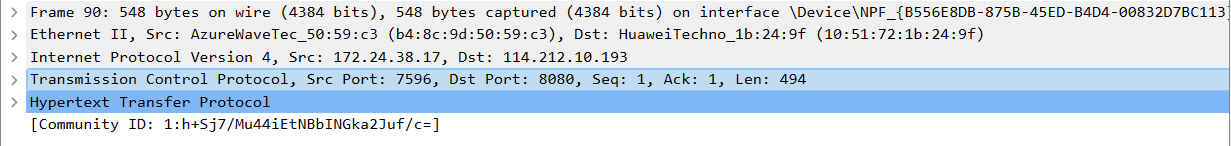
\includegraphics[width=1\textwidth]{pic0/p3.png} % 图片文件名和路径
    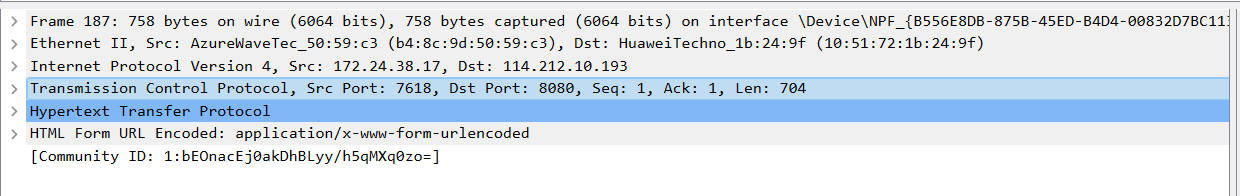
\includegraphics[width=1\textwidth]{pic0/p4.png} % 图片文件名和路径
\end{figure}

4.
\newpage
%\tu[height=0.9\textheight]{lab0.1.pdf}
\begin{figure}[htbp]
    \centering
    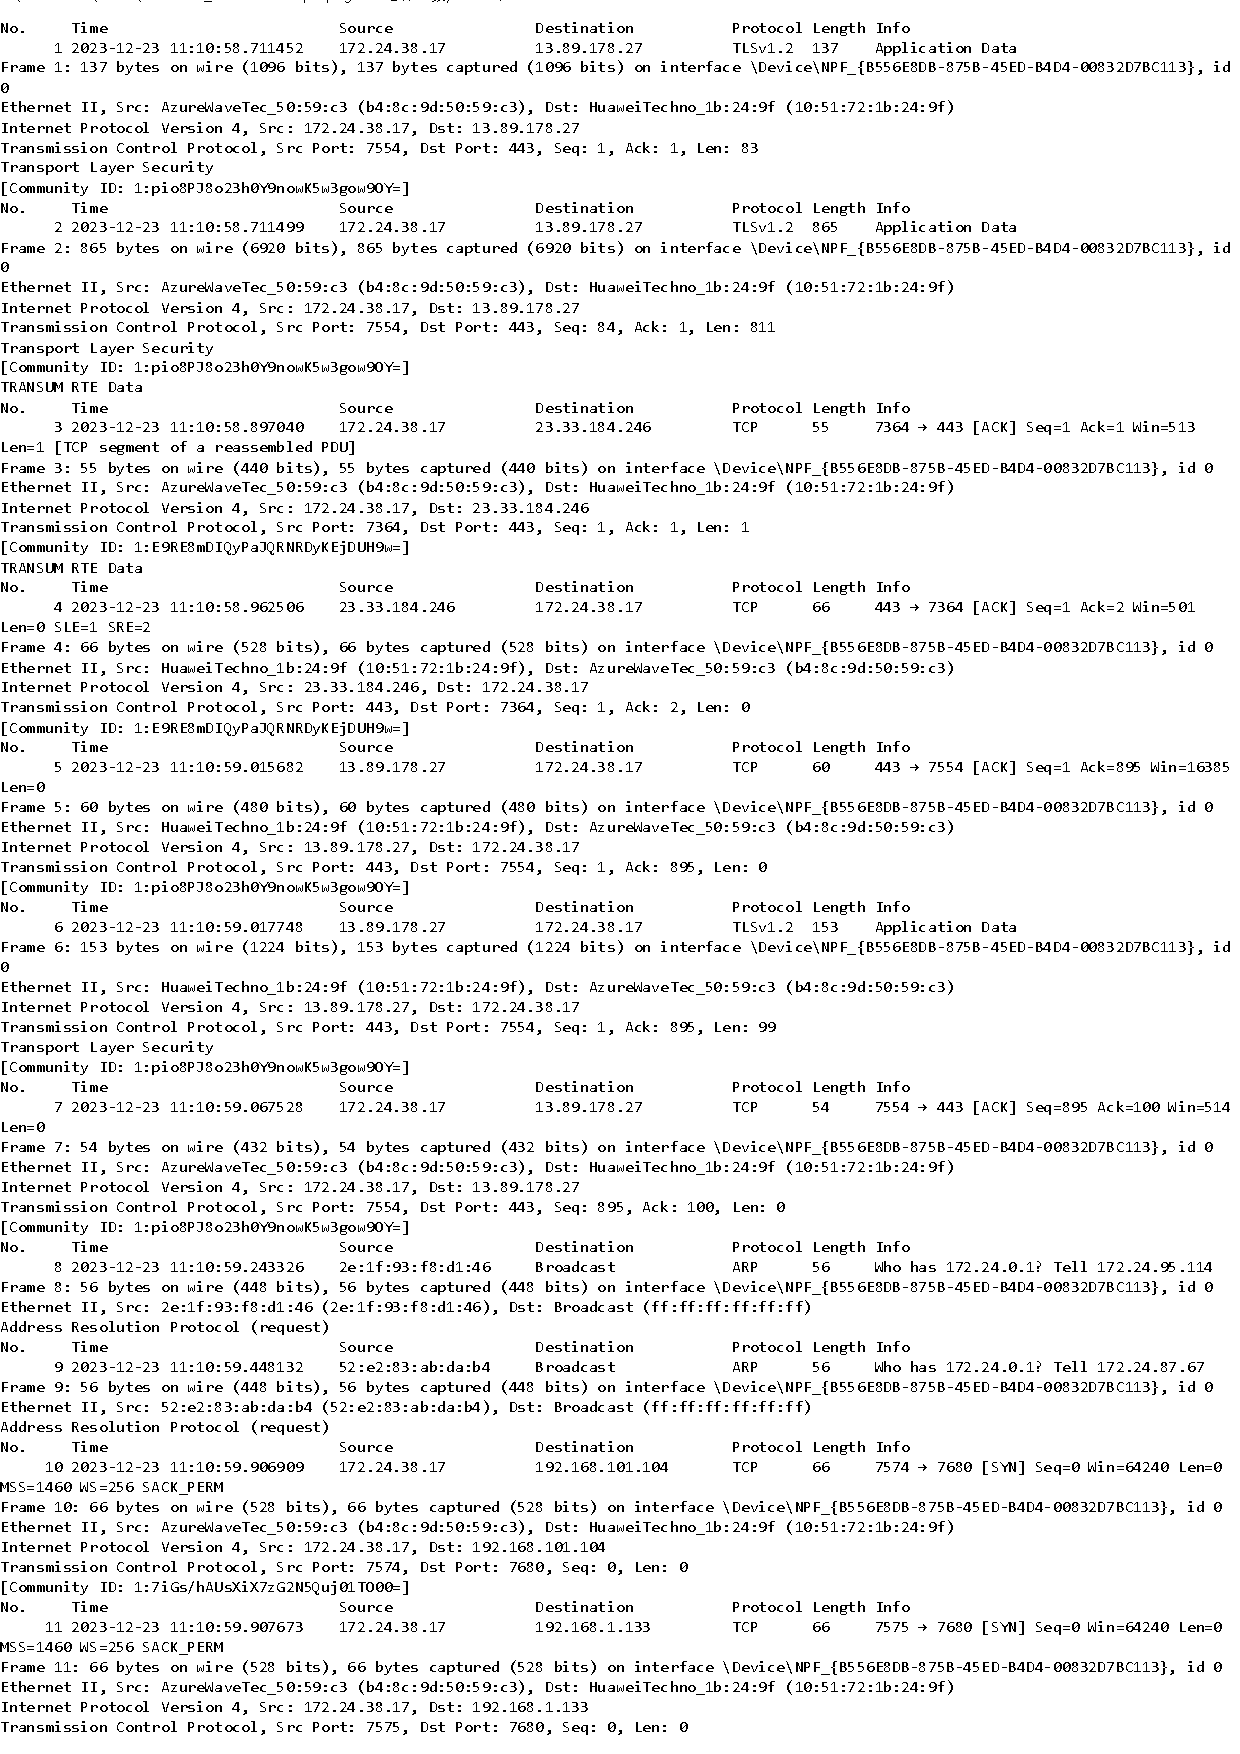
\includegraphics[width=1\textwidth]{lab0.2.pdf} % 图片文件名和路径
    %加个图片标注
    \caption{Post报文}
\end{figure}
\newpage
%\tu[height=0.9\textheight]{lab0.2.pdf}
\begin{figure}[htbp]
    \centering
    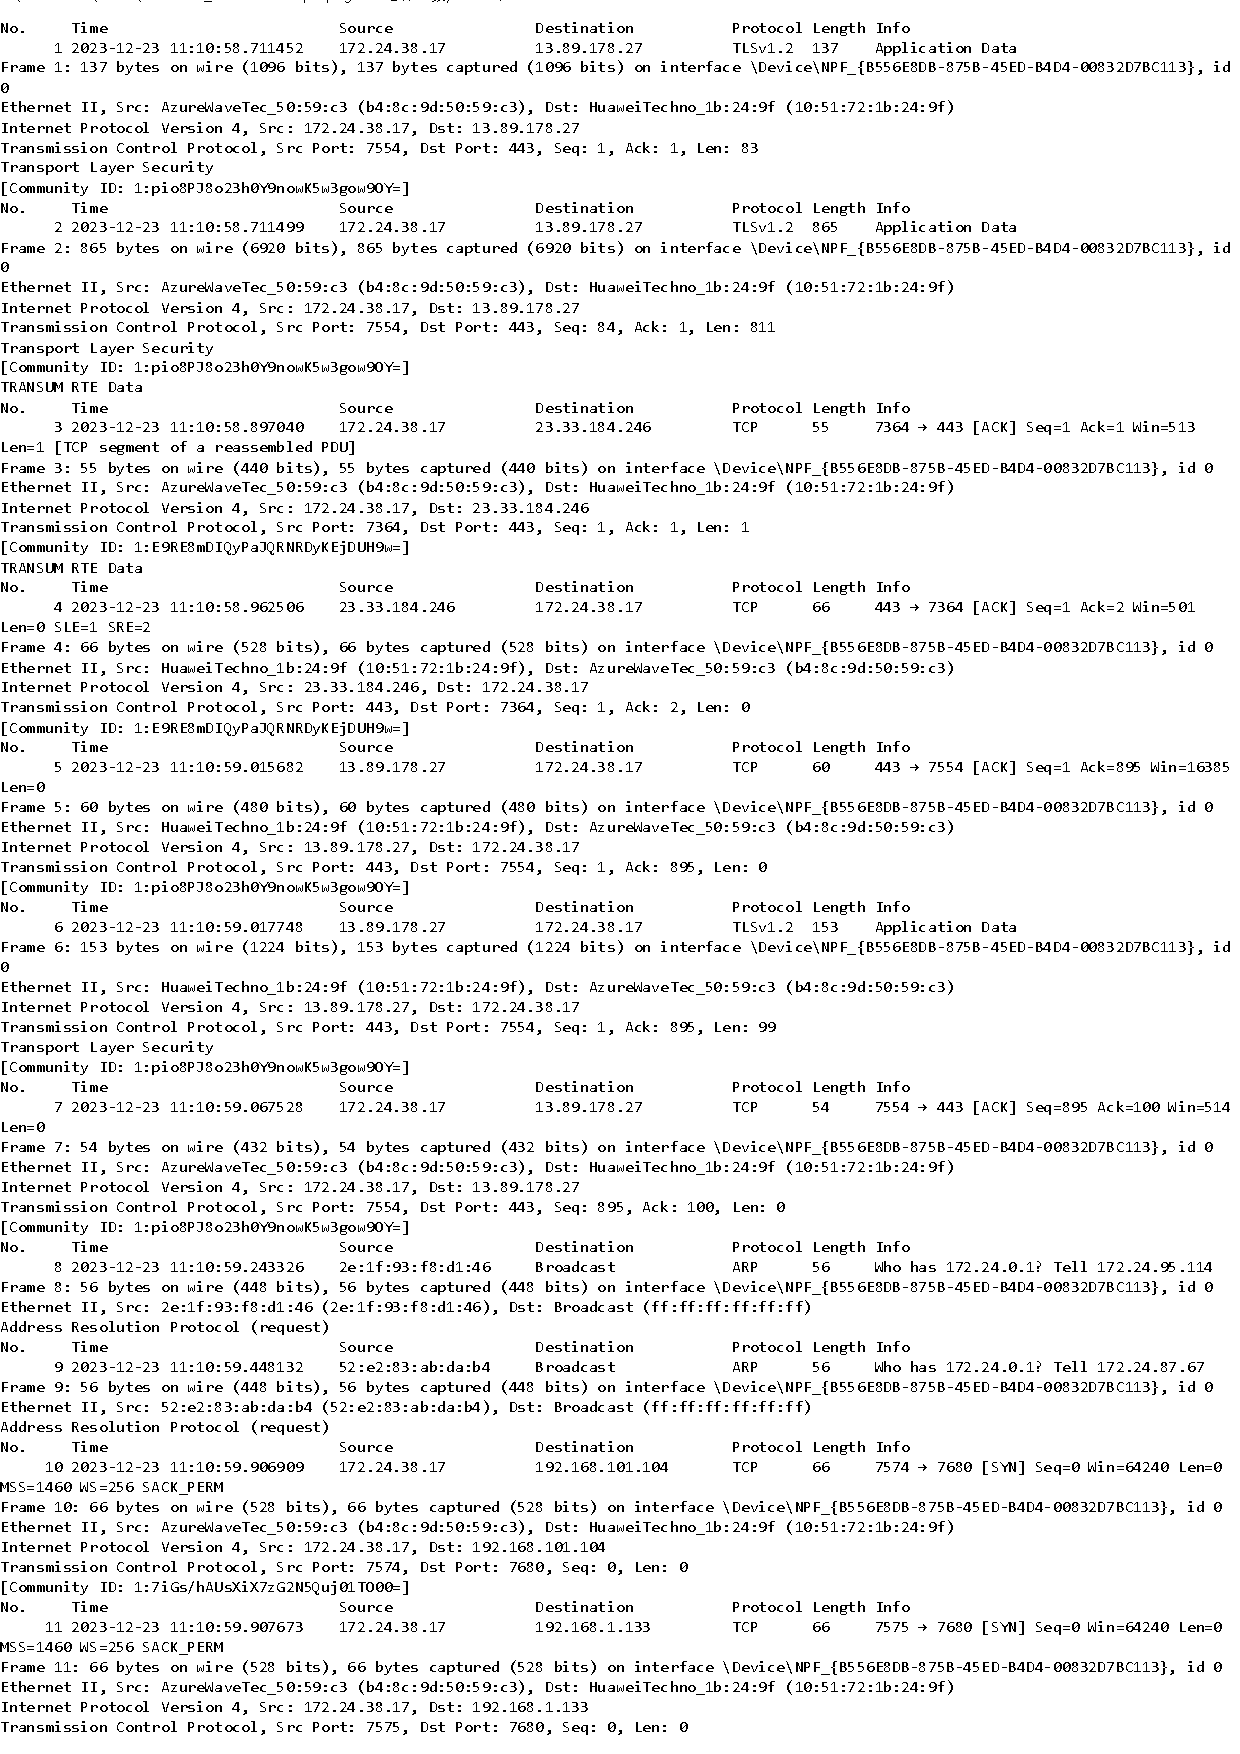
\includegraphics[width=1\textwidth]{lab0.3.pdf} % 图片文件名和路径
    %加个图片标注
    \caption{OK报文}
\end{figure}
\end{document}